\documentclass[a5paper]{article}
\usepackage[a5paper, top=8mm, bottom=8mm, left=8mm, right=8mm]{geometry}

\usepackage{polyglossia}
\setdefaultlanguage[babelshorthands=true]{russian}

\usepackage{fontspec}
\setmainfont{FreeSerif}
\newfontfamily{\russianfonttt}[Scale=0.7]{DejaVuSansMono}

\usepackage[font=scriptsize]{caption}

\usepackage{amsmath}
\usepackage{amssymb,amsfonts,textcomp}
\usepackage{color}
\usepackage{array}
\usepackage{hhline}
\usepackage{cite}

\usepackage[hang,multiple]{footmisc}
\renewcommand{\footnotelayout}{\raggedright}

\PassOptionsToPackage{hyphens}{url}\usepackage[xetex,linktocpage=true,plainpages=false,pdfpagelabels=false]{hyperref}
\hypersetup{colorlinks=true, linkcolor=blue, citecolor=blue, filecolor=blue, urlcolor=blue, pdftitle=1, pdfauthor=, pdfsubject=, pdfkeywords=}

\usepackage{tabu}

\usepackage{graphicx}
\usepackage{indentfirst}
\usepackage{multirow}
\usepackage{subfig}
\usepackage{footnote}
\usepackage{minted}

\sloppy
\pagestyle{plain}

\title{Юнит-тестирование и системы сборки}
\author{Юрий Литвинов\\\small{yurii.litvinov@gmail.com}}

\date{16.01.2019}

\begin{document}

\maketitle
\thispagestyle{empty}

\section{Введение}

На этой паре будет быстрая ликвидация безграмотности в области сопутствующих разработке любого сколько-нибудь большого проекта вещей --- модульного тестирования и организации сборки. В общем-то, каждая из этих тем заслуживает отдельной пары, но, как я понимаю, вам уже скоро надо будет приступать к написанию проектов под Android, поэтому расскажу кратко и только то, что нужно, чтобы взять и начать пользоваться. Остальное можно почитать в литературе, по мере использования этих вещей в своих проектах.

\section{Юнит-тестирование}

Во-первых, зачем нужно юнит-тестирование: есть шуточные аксиомы, которые формулируются так:
\begin{itemize}
	\item Любая программа содержит ошибки
	\item Если программа не содержит ошибок, их содержит алгоритм, который реализует эта программа
	\item Если ни программа, ни алгоритм ошибок не содержат, такая программа даром никому не нужна
\end{itemize}

В общем-то, практика показывает, что так оно и есть. Hello world можно написать и без ошибок, однако практическая ценность такой программы сомнительна. А любая достаточно сложная программная система ошибки в том или ином виде содержит. Надеяться на то, что вы умнее всех, и если будете кодить внимательно и осторожно, сумеете избежать ошибок --- глупо. Даже очень опытные программисты, если просто напишут пару сотен строк кода, они, скорее всего, не будут даже компилиться, не то что уж работать правильно. Статистика, подтверждаемая различными источниками (например, Канер, ``Тестирование программного обеспечения'') говорит, что после передачи на тестирование на 100 строк кода приходится от 1 до 3 ошибок, а при разработке допускается вообще несколько ошибок на одну строку кода (большинство --- опечатки, и тут же исправляется). При этом если ошибка выявлена и исправлена, скорее всего, она исправлена неправильно или исправление ломает ещё что-то --- опять же, по Канеру,еЕсли для исправления ошибки надо изменить не более 10 операторов, с первого раза это делают правильно в 50\% случаев, а если для исправления ошибки надо изменить не более 50 операторов, с первого раза это делают правильно в 20\% случаев. Понятно, что необходимы тесты, кроме того, необходимы регрессионные тесты --- тесты, которые проверяют, что единожды выявленная и исправленная ошибка больше не проявится в проекте. Однако с тестами есть большая проблема --- оттестировать всё невозможно. Программа из сотни строк может иметь $10^{18}$ путей исполнения, покрыть их все ни автоматическими, ни, тем более, ручными тестами не хватит времени жизни вселенной. А если хоть один путь исполнения не покрыт, именно на нём может воспроизвестись ошибка.

Обратите внимание, первым барьером на пути ошибок является компилятор --- если в программе написана явная чушь, компилятор это заметит и отругается. Разработчики языков программирования стараются сделать так, чтобы возможно большее количество ошибок обнаруживалось компилятором (или какими-то другими средствами статического анализа), потому как ошибка, дожившая до времени выполнения, может до времени и не проявляться. Поэтому, собственно, современные языки так сложны --- они намеренно ограничивают возможности программиста, чтобы не дать тому допускать ошибки, которых можно было бы избежать. Надо помогать в этом компилятору, накладывая возможно более жёсткие ограничения на программу (например, минимизируя области видимости и используя константы).

Тестирование бывает модульным --- когда тестируются отдельные модули (функции, методы, классы, и т.д.), интеграционное (когда тестируется взаимодействие набора модулей системы), и системное (когда тестируется вся система целиком, в рабочих условиях). Интеграционное тестирование и системное тестирование обычно выполняются специально обученными людьми, а вот модульное тестирование --- самими программистами. Модульное тестирование заключается в том, что для каждого класса и каждого его нетривиального метода пишутся свои тесты, которые проверяют, что метод работает как надо. Предполагается, что модульные тесты будут запускаться после каждой сборки программы, поэтому они должны работать по возможности быстро. Принято не продолжать разработку, если есть хотя бы один не прошедший модульный тест.

\subsection{Почему модульные тесты полезны}

\begin{itemize}
	\item Они помогают найти кучу ошибок на ранних этапах. Если тесты запускаются достаточно часто, вы будете помнить, что вы такое поменяли, после чего тесты перестали проходить.
	\item Тест --- это способ вызвать кусок функциональности, который вы разрабатываете, до того, как будет готово всё остальное.
	\item Тесты облегчают рефакторинг. Вы что-то поменяли, что не должно отразиться на наблюдаемом поведении вашего класса или метода, запускаете тесты и смотрите, что они действительно все прошли. 
	\item Тесты можно рассматривать как документацию к коду --- любой, кто захочет воспользоваться вашим классом, может посмотреть в ваши юнит-тесты к этому классу и посмотреть, как его использовать.
	\item Тесты помогают улучшить структуру программы --- дикую мешанину невозможно толком оттестировать, так что волей-неволей придётся задуматься об аккуратной архитектуре.
\end{itemize}

\subsection{Юнит-тесты на Java}

Модульное тестирование на Java осуществляется с помощью библиотеки jUnit, разработанной Эрихом Гамма и Кентом Беком (членами ``банды чётырёх'', они же писали книжку про паттерны и вообще активно пропагандировали ООП, Java, Agile и подобные вещи). Идея очень проста ---  каждому классу соответствует класс с таким же именем + Test на конце, который содержит тесты для всех методов класса. Есть программа, которая умеет последовательно запускать все тесты в тестовом классе и как-то обрабатывать результат. Сейчас такая штука обычно встроена в IDE, но принцип, как и в ранних версиях, такой --- если все тесты прошли, загорается зелёная полоска, если хоть один не прошёл --- красная, и пишется информация, какой тест не прошёл и почему. Сами тесты --- это просто методы тестового класса, помеченные специальной аннотацией @Test, имя их обычно позволяет судить о том, что и в какой ситуации тестируется, и что ожидается (см. \url{http://stackoverflow.com/questions/155436/unit-test-naming-best-practices}), а внутри что-то делается (готовятся данные), вызывается метод, который хотим протестировать, и смотрим на результат --- вызывая специальные методы типа assertEquals, fail и т.д. В общем, идея простая, но хорошая, поэтому jUnit была переписана на очень многих языках, в том числе для .NET --- там она называется NUnit, для С++ прямой порт не сделать, потому что там рефлексии нет, но аналогов полно --- Google Testing Framework, CppUnit, CxxTest и т.д. Несложная система модульного тестирования пишется за выходные, а особо сложных и не бывает.

Актуальная версия jUnit --- JUnit 5, однако JUnit 4 всё ещё очень популярен и иногда используется по умолчанию некоторыми инструментами, что может вас путать. IDEA про JUnit 5 знает и отлично с ним интегрируется --- умеет автоматически генерировать заглушки для тестов, запускать тесты прямо из редактора, подставлять нужные зависимости в проект и т.д.

С технической точки зрения тест --- это отдельный класс, в котором есть методы, помеченные аннотацией \mintinline{java}|@Test|. Все остальные методы --- это обычные методы класса, у класса также могут быть поля, всё это системой юнит-тестирования игнорируется, но может быть использовано из тестов. Тестовые классы могут наследоваться друг от друга, и вообще, к разработке тестов применимы те же правила, что и к разработке обычного кода (например, никакого копипаста).

Любой тест обычно состоит из трёх фаз:
\begin{itemize}
	\item настройка тестового окружения, где мы переводим тестируемый класс в состояние, которое ожидается на начало теста (например, если мы хотим потестить метод pop() у стека, надо в него что-то положить);
	\item выполнение действия, которое хотим тестировать (в нашем примере --- собственно вызываем pop());
	\item проверка результатов --- это вызовы библиотечных методов assertEquals, assertNull, assertTrue и т.д., которые, собственно, сравнивают то, что получилось, с нашими представлениями о том, что должно быть.
\end{itemize}

\subsection{Демонстрация}

Сделаем небольшой проект и юнит-тесты для него (кстати, юнит-тесты обязательны для каждой задачи в домашке). Создаём новый проект в IDEA, пишем там что-нибудь, что можно тестировать (например, факториал):

\begin{minted}{java}
package com.example;

public class Main {
    public static int factorial(int n) {
        if (n <= 1) {
            return 1;
        }

        return n * factorial(n - 1);
   }

   public static void main(String[] args) {
   }
}
\end{minted}

Дальше позволяем IDEA сделать всё за нас: ставим курсор на класс Main, жмём Alt-Enter, выбираем Create Test. Выбираем JUnit5,  выбираем методы, для которых надо сгенерить тесты, получаем что-то такое:

\begin{minted}{java}
package com.example;

import org.junit.jupiter.api.Test;

import static org.junit.jupiter.api.Assertions.*;

class MainTest {

    @Test
    void factorial() {
    }
}
\end{minted}

Теперь можно писать, собственно, тесты, используя статические методы класса Assert, который мы для удобства статически импортируем:

\begin{minted}{java}
package com.example;

import org.junit.jupiter.api.Test;

import static org.junit.jupiter.api.Assertions.*;

class MainTest {

    @Test
    void factorial() {
       assertEquals(120, Main.factorial(5));
    }
}
\end{minted}

Запускаем тест кнопкой рядом с тестом, убеждаемся, что он проходит. Портим факториал, убеждаемся, что тест не проходит больше. Обратите внимание на @Test --- это атрибут, по которому система запуска тестов JUnit знает, какие методы надо запустить. Ещё обратите внимание, что вообще не нужен метод main --- каждый тест может служить точкой входа (запускаемым методом). В нашем курсе задания, где в условии не напиано явно, что должно запускаться из консоли, могут содержать только реализацию и набор тестов, без main-а.

\subsection{Некоторые подробности}

Какие ещё аннотации бывают:
\begin{itemize}
	\item \mintinline{java}|@BeforeEach| --- метод, запускающийся перед каждым тестом;
	\item \mintinline{java}|@AfterEach| --- метод, запускающийся после каждого теста;
	\item \mintinline{java}|@BeforeAll| --- метод, запускающийся перед всеми тестами в классе (должен быть static);
	\item \mintinline{java}|@AfterAll| --- метод, запускающийся после всех тестов в классе (должен быть static);
	\item \mintinline{java}|@Disabled| --- тест отключён и не запускается.
\end{itemize}

Бывают и ещё разные аннотации, имеет смысл посмотреть документацию на JUnit (хотя большая часть интересных вещей пока экспериментальная).

Вот основные assertion-ы, которые могут пригодиться.

\begin{itemize}
	\item assertEquals проверяет на равенство два элемента. Метод имеет перегрузки для примитивных типов и вызывает equals ддля остальных, поэтому правильно работает со строками, типами-обёртками, и вообще, скорее всего, будет вести себя ожидаемо. Обратите внимание на порядок параметров, сначала то, что мы ожидаем получить, затем реальное значение --- то, что получилось в ходе теста.
	\item assertArrayEquals проверяет на равенство два массива, вызывая assertEquals для каждого элемента. Сравнивать массивы можно только так, assertEquals проверит равенство только ссылок.
	\item assertTrue/assertFalse проверяет истинность/ложность переданного ему утверждения.
	\item assertNull/assertNotNull проверяет, что переданная ему ссылка null или не null.
	\item assertThrows проверяет, что переданная функция (метод или лямбда) бросили в процессе работы исключение правильного типа. Да, исключения тоже надо проверять.
	\item fail просто помечает тест как непройденный. Редко нужен, потому что есть методы assert-что-нибудь.
\end{itemize}

Последнее, про что хочется упомянуть --- это best practices юнит-тестирования:

\begin{itemize}
	\item тесты должны быть независимыми, то есть в идеале одна поломка в коде должна ломать один тест;
	\item имеет смысл изолировать тестируемые объекты, для этого могут применяться mock-объекты (полезно погуглить, но про это ещё будет);
	\item тесты должны работать быстро;
	\item тесты должны запускаться часто, как минимум, перед каждым коммитом (либо после коммита на сервере непрерывной интеграции);
	\item тесты должны проверять конкретный сценарий работы системы, никаких try-catch в коде теста быть не должно, используйте assertThrows; то же касается тестов с элементами случайности --- они могут быть полезны, но их трудно воспроизвести, а надёжная воспроизводимость необходима, чтобы исправить ошибку;
	\item тестов должно быть много (погуглите про coverage, либо я потом покажу);
	\item тесты должны называться говорящими именами --- в какой ситуации мы находимся, что проверяем и что ожидаем. Например, shouldReturnLastPushedValueWhenCallingPop() для стека. Не надо бояться длинных имён тестов, потому что когда у вас в реальном проекте будет несколько тысяч тестов и пять из них не пройдут, вам будет гораздо приятнее читать лог ночной сборки, если тесты будут иметь адекватные имена, а не что-нибудь вроде test239().
	\item Есть известная методология разработки, Test-Driven Development (TDD), когда сначала пишутся тесты, а потом код. Кажется бредом, потому что раз кода нет, что же тестировать --- но на самом деле, написание теста позволяет уточнить требования к коду, который мы ещё только собираемся писать, и лучше понять задачу. После того, как тест написан, убеждаемся, что он не проходит, пишем код, убеждаемся, что тест проходит, рефакторим код. Продолжаем так до тех пор, пока не сможем больше придумать содержательных тестов. Не пишем код, для которого нет теста, даже если ``это на будущее'', ``это для красивой архитектуры'' и т.д.
\end{itemize}

\section{Системы сборки}

Следующее семейство технологий, которое используется во всех больших проектах --- это системы сборки. Они нужны для автоматизации сборки приложения, которая в больших проектах может быть чрезвычайно сложной процедурой, состоящей из нескольких фаз сборки исходников, сборки инсталляторов, сборки документации, деплоя (возможно, на удалённый сервер, а возможно, на целую инфраструктуру серверов), различных манипуляций с ресурсами, запуска юнит-тестов и т.д. Нередки проекты, в которых сборка идёт несколько часов. Я работал в проекте, где сборка требовала запуска трёх виртуалок, сборки отдельной части проекта кросскомпилятором и выкладывания её в гит, укачивания из гита её и ещё парочки заранее собранных компонентов, включения в инсталлятор вместе с только что собранными под конкретную ОС исходниками и заливки инсталлятора (инсталляторов под 4 поддерживаемые ОС, на самом деле) на сервер репозитория для рассылки автообновлений. Если делать это вручную, можно сойти с ума, к тому же, велика вероятность совершить ошибку и выложить в продакшн что-то не то.

Есть распространённое заблуждение, что среда разработки и так вам всё соберёт. Но если вы собираете проект только локально, может оказаться так, что только у вас этот проект и собирается. Кроме того, сборка может зависеть от локальных настроек, локальных переменных окружения, конкретных версий конкретных инструментов и библиотек, установленных на конкретной машине, то есть может быть нарушена воспроизводимость сборки, что для любого нормального проекта, естественно, недопустимо. Чтобы этого избежать, придумали Continious Integration --- отдельный билд-сервер, подписанный на сообщения о коммитах и собирающий проект после каждого коммита автоматически (и запускающий юнит-тесты, кстати). Есть несколько таких бесплатных для опенсорс-проектов штук в облаке, например, Travis или AppVeyor. На билд-сервере никакой IDE нет, всё должно запускаться из командной строки.

Типичная система сборки (например, make) умеет выполнять некоторые действия для сборки проекта в правильном порядке, действия обычно называются задачами, а порядок определяется зависимостями между задачами (например, нет смысла запускать юнит-тесты, если проект ещё не собран). Система сборки строит граф задач и выполняет на нём топологическую сортировку, после чего начинает последовательно исполнять задачи, передавая, возможно, результаты одной как входные параметры другой. Всё это управляется конфигурационным файлом сборки, где задачи могут быть описаны явно (как это надо было делать в make) или декларативно (как в Maven). Задачи могут быть не только вызовами компилятора, с помощью систем сборки можно автоматизировать любой процесс, где есть входные данные, несколько разных программ или действий, которые надо на входных данных выполнить, получить выходные данные и, возможно, выполнить на них ещё что-то (например, конвертить картинки в папке или расставлять тэги mp3-файлам вполне можно и make-ом). Этим системы сборки похожи на скрипты (bash, cmd), но в скриптах практически всё надо писать руками и результат окажется непереносимым между платформами (да даже между разными командными интерпретаторами на одной платформе).

В мире Java весьма популярны системы сборки Ant (очень похожа на make, поэтому считается отжившей свой век и deprecated), Maven и Gradle. Далее будет подробнее про две последние, благо они довольно типичные представители современных систем сборки --- обе умеют декларативно описывать проект, что нужно собрать и что для этого нужно, обе умеют подкачивать нужные зависимости прямо в процессе сборки, обе можно использовать не только для сборки, но и для других задач типа генерации документации.

\subsection{Apache Maven}

Maven --- это система сборки, которую написали, когда поняли, что на Ant надо писать кучу кода на XML, который ещё и тяжело переиспользуется между проектами (кстати, Ant появился в 2000 году, Maven --- в 2004, Gradle --- в 2008). Maven позволяет не писать действия при сборке, а позволяет описать конфигурацию сборки, остальное билд-система сделает сама (декларативный стиль описания сборки). При этом он использует подход ``Convention Over Configuration'', то есть ожидает от проекта следования некоторому набору правил и определяет ряд умолчаний, так, что если всё хорошо, то сборка требует лишь минимальной конфигурации. Вот пример минимальной конфигурации, позволяющей собрать автоматически java-исходники и тесты, после чего запустить тесты:

\begin{minted}{xml}
<?xml version="1.0" encoding="UTF-8"?>
<project xmlns="http://maven.apache.org/POM/4.0.0"
         xmlns:xsi="http://www.w3.org/2001/XMLSchema-instance"
         xsi:schemaLocation="http://maven.apache.org/POM/4.0.0 
             http://maven.apache.org/xsd/maven-4.0.0.xsd">
    <modelVersion>4.0.0</modelVersion>

    <groupId>com.example</groupId>
    <artifactId>Example</artifactId>
    <version>1.0-SNAPSHOT</version>

    <build>
        <plugins>
            <plugin>
                <artifactId>maven-surefire-plugin</artifactId>
                <version>2.22.0</version>
            </plugin>
            <plugin>
                <groupId>org.apache.maven.plugins</groupId>
                <artifactId>maven-compiler-plugin</artifactId>
                <version>3.8.0</version>
                <configuration>
                    <release>11</release>
                </configuration>
            </plugin>
        </plugins>
    </build>

    <dependencies>
        <dependency>
            <groupId>org.junit.jupiter</groupId>
            <artifactId>junit-jupiter-api</artifactId>
            <version>5.3.2</version>
            <scope>test</scope>
        </dependency>
        <dependency>
            <groupId>org.junit.jupiter</groupId>
            <artifactId>junit-jupiter-engine</artifactId>
            <version>5.3.2</version>
            <scope>test</scope>
        </dependency>
    </dependencies>

</project>
\end{minted}

Тут описывается лишь информация про проект в духе его названия и версии, выставляется версия языка Java, подключается плагин для автоматического запуска юнит-тестов после сборки, описывается зависимость от библиотеки JUnit (от двух её пакетов --- API, который следует использовать в тестах, и движка, который эти самые тесты запускает). Довольно многословно, как видим, и не вполне очевидно, что писать, но по этому делу есть куча документации, и каждый нормальный автор библиотек для Java обязательно пишет инструкции про то, как их включить в сборку на Maven. Ещё можно обратить внимание на то, что нигде нет ни последовательности действий для сборки, ни собственно того, что надо делать и откуда брать исходники --- это тот самый подход Convention Over Configuration. Если вы всё делаете как надо, всё легко, но если вы хотите делать как-то по-своему, то у вас проблемы. Например, последовательность задач, выполняемых при сборке, определяется жизненным циклом, который зафиксирован самим Maven.

Сам Maven практически ничего делать не умеет, поэтому размер установщика --- всего полтора мегабайта (вообще, он есть в установке IDEA, поэтому отдельно ставить его не нужно). Всё делается плагинами, которые подкачиваются из репозитория по мере их первого использования. Плагины интегрируются в фазы жизненного цикла сборки, которые определены в самом Maven (там есть фазы типа валидации, компиляции, запуска юнит-тестов, деплоя и т.д.). 

Ключевой для Maven файл --- это pom.xml, Project Object Model, где хранится информация о проекте и его конфигурации, о том, как его собирать, от кого он зависит, и вообще, что с ним надо делать (тот самый пример xml-ки выше). Собственно, этого файла в корне проекта достаточно, чтобы Maven мог собирать проект. При этом в POM единственная обязательная штука --- это ``координаты'' проекта, которые позволяют его однозначно идентифицировать, в том числе и глобально, если проект будет выложен в общий репозиторий. Координаты состоят из groupId --- чего-то вроде имени пакета Java, как правило, доменного имени компании --- автора приложения, artifactId --- имени самого приложения, и версии, записанной по определённой (довольно классической) схеме (<major version>.<minor version>.<release>-<modifier>). Всякие зависимости и плагины у нас в примере только потому, что мы хотим Java 11 (а не Java 6, как по умолчанию), и JUnit 5, и чтобы оно само запускалось по команде mvn install.

Координаты пакетов используются для того, чтобы Maven мог автоматически подкачивать зависимости из интернета (что выгодно отличает его от make и подобных вещей), можно просто задекларировать, что хочу JUnit такой-то версии, и при сборке Maven сам его найдёт (у себя в облачном репозитории) и скачает. Причём, скачает в локальный кеш (который лежит в ~/.m2, ~ --- это папка пользователя, которая под Windows что-то вроде  C:/Users/<пользователь>), и при последующих сборках будет использовать скачанные пакеты.

Вот стандартная структура папок Maven:

\begin{minted}{text}
pom.xml
src
    main
        java
        resources
    test
        java
        resources
target
\end{minted}

Папку target Maven создаст сам при сборке и положит туда результаты (файлы .class, .jar-архив), остальные папки надо (если надо) создать вручную. IDEA, в общем-то, тут тоже в состоянии всё сделать за вас. Если вам не нравится идея класть исходники конкретно в папку src/main/java и вы хотите положить их в mysrc/awesomeApp/javarip, то, в общем-то, Maven не для вас (его можно переубедить, но это ``против шерсти'').

\subsubsection{Демонстрация}

Создаём в IDEA новый проект, выбираем Maven, чтобы было как-то так:

\begin{center}
	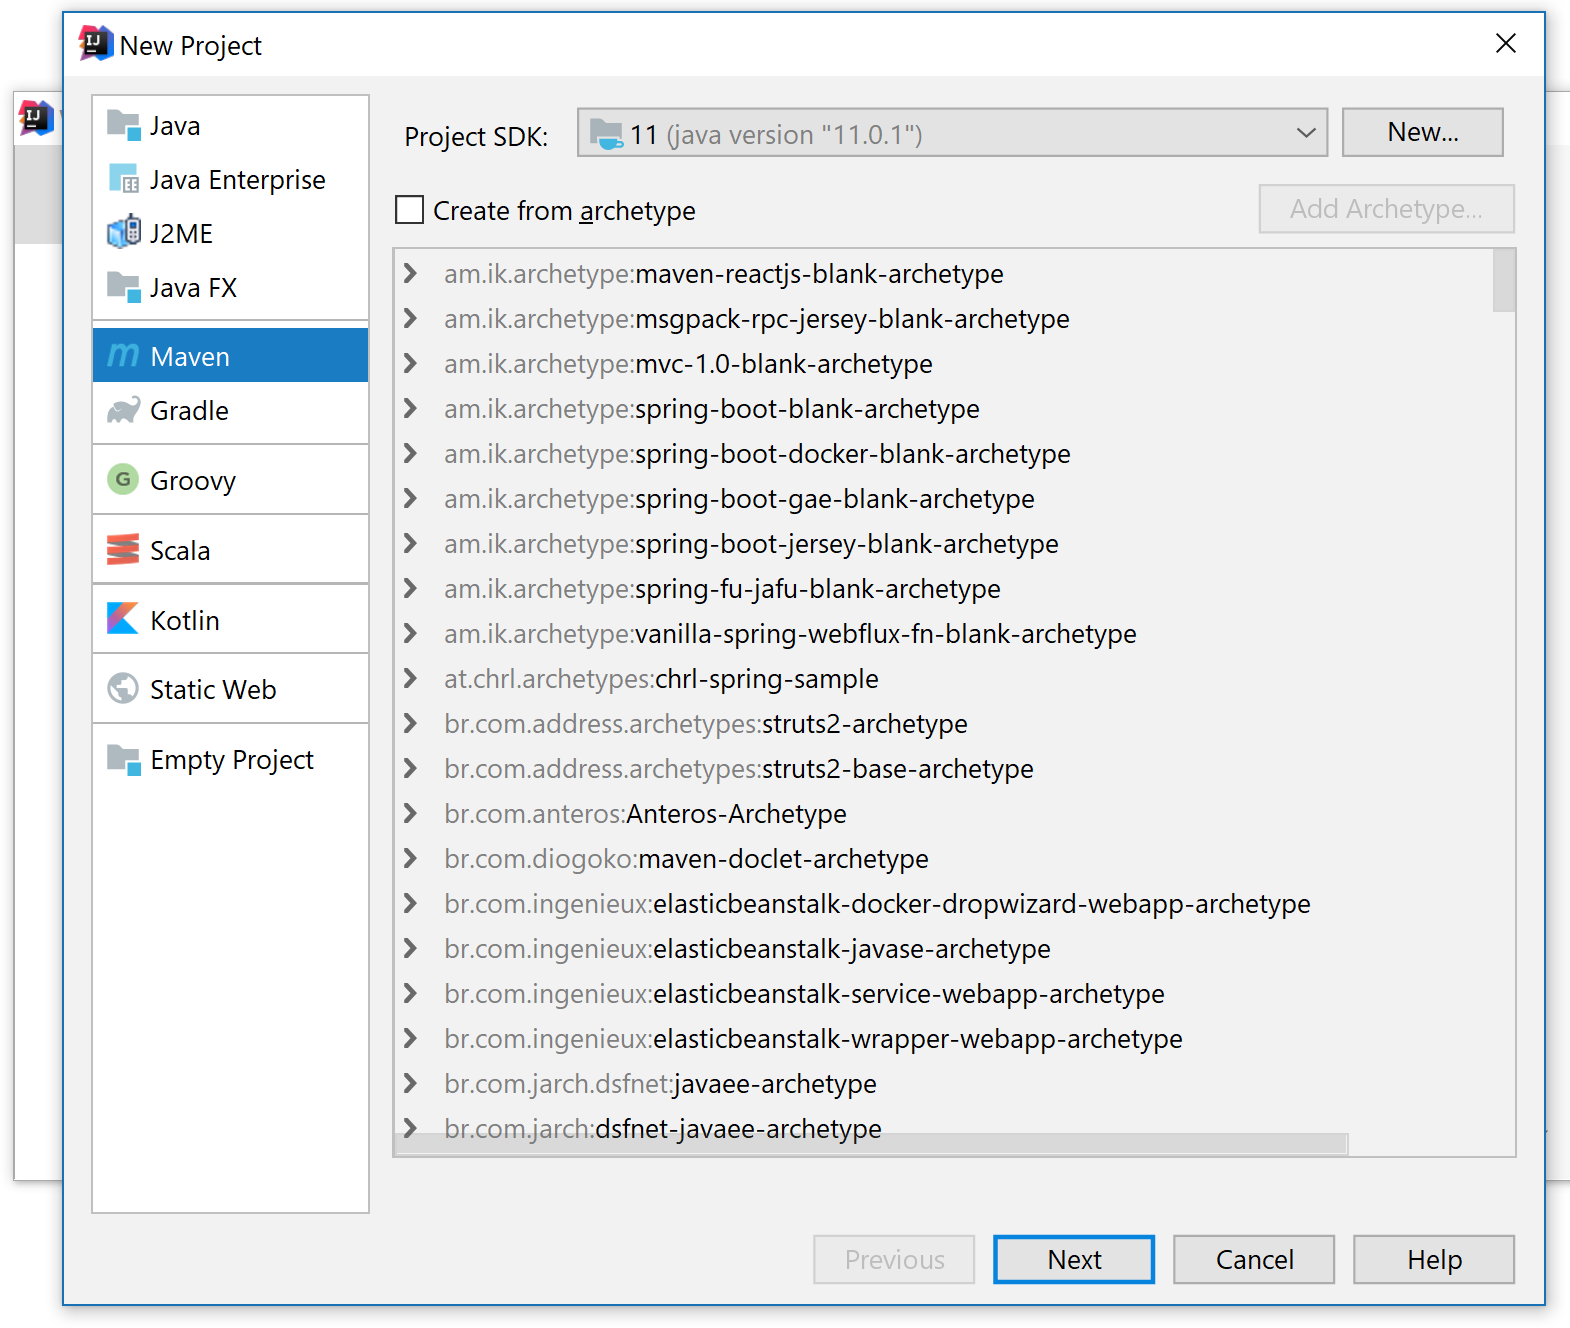
\includegraphics[width=0.8\textwidth]{mavenProject.png}
\end{center}

Жмём next, указываем в следующем окошке координаты проекта (сами их придумываем), затем --- имя проекта и его положение на диске. Сгенерируется вот такой минимальный pom.xml:

\begin{minted}{xml}
<?xml version="1.0" encoding="UTF-8"?>
<project xmlns="http://maven.apache.org/POM/4.0.0"
         xmlns:xsi="http://www.w3.org/2001/XMLSchema-instance"
         xsi:schemaLocation="http://maven.apache.org/POM/4.0.0 
             http://maven.apache.org/xsd/maven-4.0.0.xsd">
    <modelVersion>4.0.0</modelVersion>

    <groupId>com.example</groupId>
    <artifactId>Example2</artifactId>
    <version>1.0-SNAPSHOT</version>
</project>
\end{minted}

Идём в src/main/java и создаём там какой-нить класс, создаём для него юнит-тест, как было чуть выше. IDEA сама добавит в pom.xml ссылку на JUnit 5 API. Дальше обращаем внимание на незаметную кнопку Maven Projects справа. Это, собственно, фазы жизненного цикла Maven, выбираем Lifecycle/test, жмём run maven build, и оно внезапно не компилится с ообщением

\begin{minted}{text}
[ERROR] Source option 5 is no longer supported. Use 6 or later.
\end{minted}

Это довольно странный способ сообщить пользователю о том, что Maven современных версий требует явного указания версии Java в pom.xml. Окей, дописываем конфигурацию плагина, отвечающего за компиляцию, вручную:

\begin{minted}{xml}
<?xml version="1.0" encoding="UTF-8"?>
<project xmlns="http://maven.apache.org/POM/4.0.0"
         xmlns:xsi="http://www.w3.org/2001/XMLSchema-instance"
         xsi:schemaLocation="http://maven.apache.org/POM/4.0.0
             http://maven.apache.org/xsd/maven-4.0.0.xsd">
    <modelVersion>4.0.0</modelVersion>

    <groupId>com.example</groupId>
    <artifactId>Example</artifactId>
    <version>1.0-SNAPSHOT</version>

    <build>
        <plugins>
            <plugin>
                <groupId>org.apache.maven.plugins</groupId>
                <artifactId>maven-compiler-plugin</artifactId>
                <version>3.8.0</version>
                <configuration>
                    <release>11</release>
                </configuration>
            </plugin>
        </plugins>
    </build>

    <dependencies>
        <dependency>
            <groupId>org.junit.jupiter</groupId>
            <artifactId>junit-jupiter-api</artifactId>
            <version>5.3.2</version>
            <scope>test</scope>
        </dependency>
    </dependencies>
</project>
\end{minted}

Теперь всё собирается, но не запускаются тесты. Впрочем,может и не собираться, потому что Maven хочет иметь в окружении переменную JAVA\_HOME или ещё на что-нибудь ругаться, при этом IDEA не очень информативно выдаёт сообщения об ошибке. Тогда надо запустить сборку из консоли. Maven из поставки IDEA у меня лежит в папке C:\\Program Files\\JetBrains\\IntelliJ IDEA 2018.3\\plugins\\maven\\lib\\maven3\\bin, его можно добавить в переменную окружения PATH, потом в папке проекта (там, где лежит pom.xml) выполнить команду mvn install и посмотреть, что ему не понравится. Вообще, распространяемый с IDEA Maven староват, не зазорно поставить его отдельно и посвежее (тогда не забыть прописать в PATH именно его).

Чтобы тесты запускались, надо подключить maven-surefire-plugin и прописать зависимость от junit-jupiter-engine (опять-таки, к сожалению, вручную), то есть привести pom.xml к виду, показанному ещё в самом первом примере.

\subsection{Gradle}

Gradle --- это более свежая альтернатива Maven, которая появилась из-за того, что Maven слишком навязывает проектам своё видение процесса сборки и не все большие проекты могут этому видению следовать. Кроме того, xml-конфигурация Maven слишком многословна (в силу особенностей синтаксиса XML), поэтому решили использовать для написания конфигурации сборки язык программирования высокого уровня, или более конкретно, Groovy. Поскольку Gradle появился на основе опыта Maven, он использует, в общем-то, тот же подход --- Convention Over Configuration, стандартную структуру папок. Но, в отличие от Maven, он позволяет писать конфиг сборки и в императивном стиле, работая напрямую с задачами, и переопределять всё, что можно, без особой головной боли. Кроме того, Gradle позволяет пользоваться мавеновскими репозиториями и качать пакеты из них.

Собственно, конфиг сборки в Gradle описывается в файле build.gradle. Если создать новый проект, выглядит он примерно вот так:

\begin{minted}{groovy}
plugins {
    id 'java'
}

group 'com.example'
version '1.0-SNAPSHOT'

sourceCompatibility = 1.8

repositories {
    mavenCentral()
}

dependencies {
    testCompile group: 'junit', name: 'junit', version: '4.12'
}
\end{minted}

Генерится ещё файл settings.gradle, который нужен для многопроектных сборок, в нём определяется структура дерева проектов. Для сборки из одного проекта он опционален.

\subsubsection{Демонстрация}

Как обычно, создаём в IDEA новый проект, но выбираем Gradle. Дальше всё по аналогии с Maven-ом, в общем-то. Генерируется build.gradle по умолчанию, как в листинге выше. Такой конфиг нам не очень подойдёт, поскольку тут используется JUnit 4 и версия языка 8 --- всякие legacy-технологии. Перепишем по-человечески (к несчастью, вручную):

\begin{minted}{groovy}
plugins {
    id 'java'
}

group 'com.example'
version '1.0-SNAPSHOT'

sourceCompatibility = 11

repositories {
    mavenCentral()
}

dependencies {
    testCompile('org.junit.jupiter:junit-jupiter-api:5.3.2')
    testRuntime('org.junit.jupiter:junit-jupiter-engine:5.3.2')
}

test {
    useJUnitPlatform()
}
\end{minted}

Нажмём на Import Changes во всплывающем окошке справа внизу (это заставит IDEA синхронизировать свои проектные файлы с тем, что написано в конфиге сборки), откроем окно Gradle на панели справа, откроем там Tasks -> build и запустим задачу build. И оно, как это принято, не соберётся, сказав, что не знает никакой Java 11. Потому что с IDEA поставляется Gradle 4, которая вышла до Java 11 и правда о ней не знает. Надо вручную поставить Gradle 5 (ну, относительно вручную, через пакетный менеджер в Linux-подобных ОС и... тоже через пакетный менеджер, например, Chocolatey, в Windows) и сказать в File -> Settings -> Build, Execution, Deployment -> Gradle, что мы хотим Use local distribution (с некоторой вероятностью IDEA сама подставит сюда путь до Gradle).

Чтобы так не мучить пользователей, которые хотят просто собрать и запустить проект, у Gradle есть интересная функциональность, gradle-wrapper. Это небольшая Java-программа плюс набор скриптов, задача которых --- скачать дистрибутив Gradle правильной версии и запустить сборку, не заморачивая пользователя установкой Gradle и настройкой IDEA. То есть система сборки выкачивает сама себя в процессе сборки, такие дела. Чтобы так сделать, надо таки один раз поставить себе Gradle, прописать его в PATH, пойти в папку с проектом и набрать в командной строке gradle wrapper. Эта команда установит в проект gradle-wrapper, то есть создаст папку gradle/wrapper, где будут файлы gradle-wrapper.jar и gradle-wrapper.properties, и в корне проекта создадутся файлы gradlew и gradlew.bat. Все эти четыре файла коммитим в гитовый репозиторий (обратите внимание, .jar-файлы часто добавляются в .gitignore, gradle-wrapper.jar нужно прописать как исключение; кто не знает, о чём это, на следующей неделе расскажу). Теперь для сборки на любой машине, где есть JDK 11, достаточно сделать git clone и gradlew build. Оно само всё скачает и соберёт.

Отныне в домашке будет требоваться, чтобы всё собиралось из консоли одной командой --- либо mvn install, либо gradlew build. Проще всего проверить, что всё ок, склонив репозиторий в чистую папку и исполнив одну из этих команд. Или настроить CI, если умеете.

\end{document}
